\section{Software} \label{sec:software}

Die Software ist als Model-View-Controller Entwurf aufgebaut. Diese Struktur wird im Anhang erläutert. Somit sind die Berechnungen von der Benutzeroberfläche getrennt. Während im Model die Schaltbilder aufgebrochen werden um die Einfügedämpfung zu berechnen wird die Benutzeroberfläche in einzelne Panels aufgeteilt. Diese Panels beinhalten jeweils eine Grundfunktion der Software. Im Klassendiagramm (Abbildung \ref{fig:klassendiagramm} ) sind die Inhalte der verschiedenen Programmteile, sowie deren zusammenspiel ersichtlich. Der Controller wird standardmässig nur zur Übergabe der Befehle zwischen View und Model verwendet. Ausserhalb dieser Struktur befindet sich noch das Framework, welches die gesamte Software intialisiert. Im Klassendiagramm sind auch noch weitere externe Klassen vorhanden, welche der Software verschiedene Methoden zur Verfügung stellen. Diese gehören nicht zum MVC Entwurf da sie allgemeingültig sind und nicht für ein spezifisches Problem erstellt wurden.


\begin{figure}[H]
		\centering
		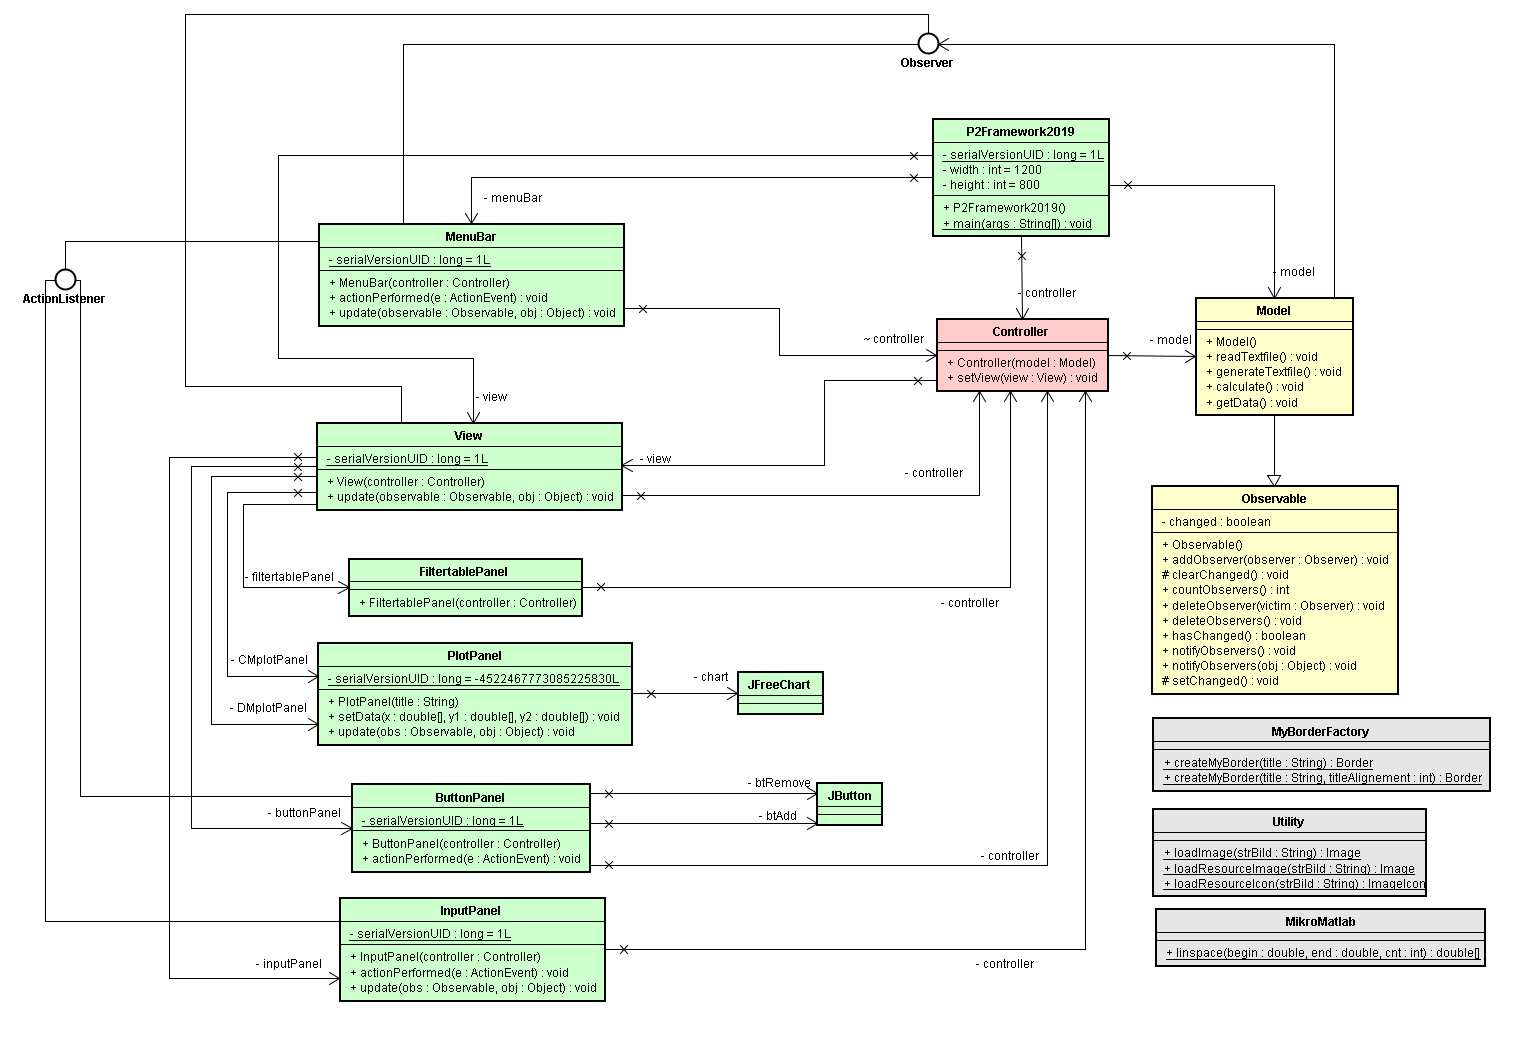
\includegraphics[width = 16cm]{Klassendiagramm.png}
		\label{fig:klassendiagramm}
		\caption{Klassendiagramm}
\end{figure}

\subsection{Ermittlung der Einfügedämpfung} \label{subsec:ermittlung}
Aufbrechen der Schaltung, beschrieb der Klassen und Methoden des Models

\begin{figure}[H]
	\begin{minipage}[h]{0.45\linewidth}
		\centering
		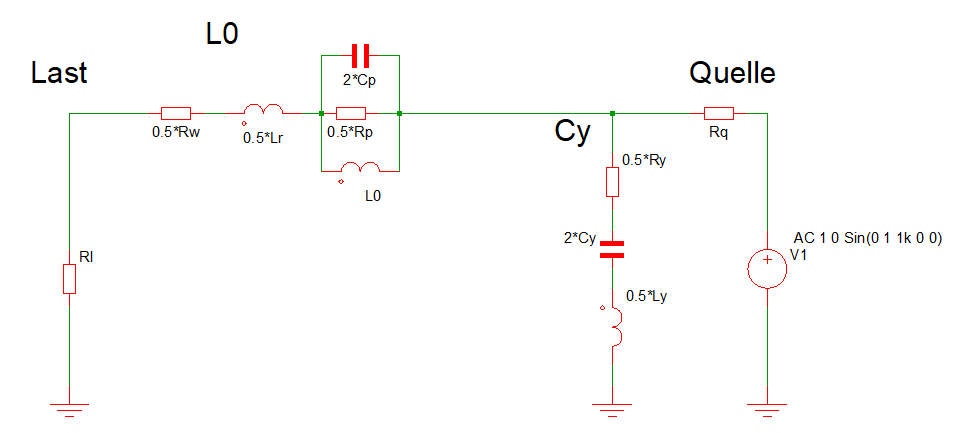
\includegraphics[width = 6cm]{EMI_CM.png}
		\label{fig:piImpedance}
		\caption{Vereinfachte \cite{CM_Schaltung}}
	\end{minipage}
\end{figure}

\begin{figure}[H]
	\begin{minipage}[h]{0.45\linewidth}
		\centering
		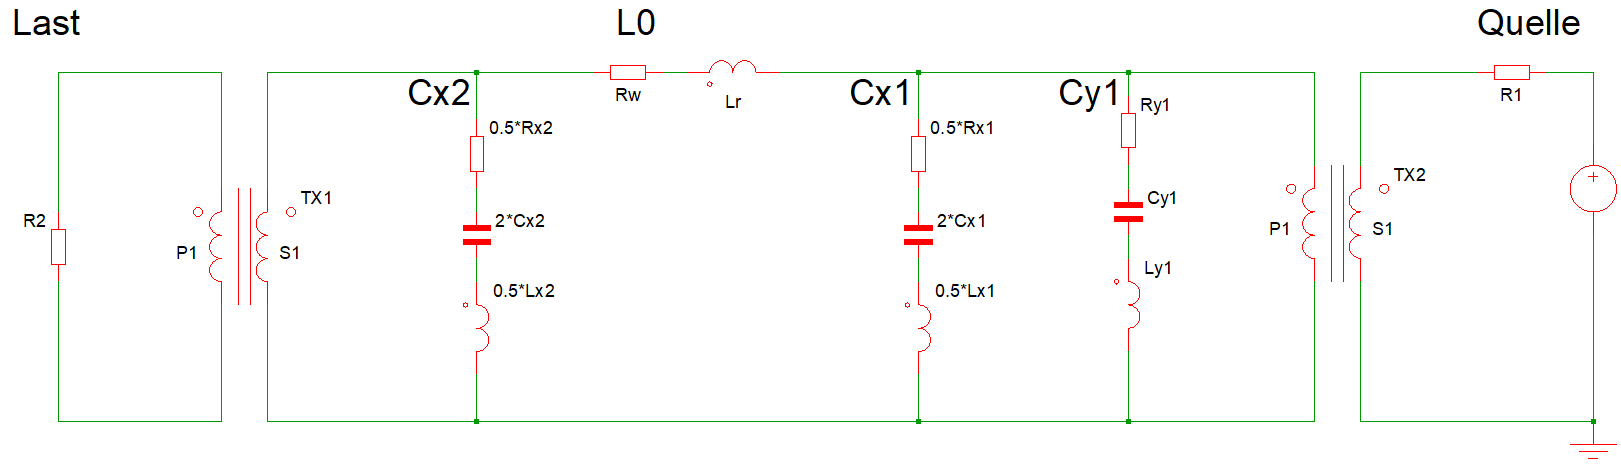
\includegraphics[width = 6cm]{EMI_DM.png}
		\label{fig:piImpedance}
		\caption{Vereinfachte \cite{DM-Schaltung}}
	\end{minipage}
\end{figure}


\subsection{Benutzeroberfläche} \label{subsec:benutzeroberflaeche}
Aufbau unserer GUI zeigen, Datenverarbeitung aufzeigen und Zusammenspiel der Panels erklären

Danach subsub's der einzelnen Panels um deren Funktionen zu zeigen


\subsubsection{Plotpanel} \label{subsubsec:plotpanel}



\subsubsection{Menu}\label{subsubsec:menu}


\subsubsection{Inputpanel} \label{subsubsec:inputpanel}


\subsubsection{Filtertabelle} \label{subsubsec:filtertabelle}





